\chapter{Nuclear structure}

\section{Spin flipping and Mossbauer}

In Mossbauer spectroscopy the nuclear decay of $Cobalt^{57}$ to $Fe^{57}$ is often used: $Co^{57} \Rightarrow Fe^{57}$.
A good introduction is by prof Guetlich \cite{Guetlich}.

Figure~\vref{fig:nuclear_decay_scheme_57fe_mossbauer} shows the different energy levels and the energies of the emitted photons.


\begin{figure}[!ht]
    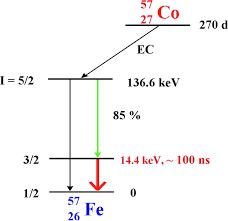
\includegraphics{nuclear_decay_scheme_57fe_mossbauer.png}
    \caption{Nuclear decay scheme 57fe Mossbauer\label{fig:nuclear_decay_scheme_57fe_mossbauer}}
    
\end{figure}


\includepdf[ pages={12,40,82,90} , nup=2x2, frame]{./bib/Cited_webpages_copy/Moessbauer_Lectures.pdf}


$^{57}Co$ has a spin of $\sfrac{7}{2}$, so in our model it has at least 7 long ornac-sticks with three nucleids. These are oriented in about the same direction to create the magnetic moment.
$Co^{57}$ has 27 protons and 30 neutrons, so of the 7  long ornac-sticks three are from the surplus of neutrons, so thrice $1p+2n$, these are Tritium sticks. 

The other four are made up by a combination of twice $2p+1n$ and twice $1p+2n$. So a total of two Hetrium sticks and five Tritium sticks.

\paragraph{}
$Co^{57}$  decays by electron capture: one of the Hetrium sticks captures the electron and transforms into a Tritium stick. The transform from hetrium to tritium lets the magnetic field flip in orientation. So $Fe^{57}$ in its first state has a spin of $I = \sfrac{5}{2}$.

So we can conclude that $Fe^{57}$ has at least 7 long ornac-sticks of which one is a Hetrium stick.
This decays quickly into $Fe^{57}$ $\sfrac{3}{2}$. This happens by a rearrangment of the long ornac-sticks: one of them flips direction so it cancels the magnetic field of one other stick.

\paragraph{}
Another thing is that there is the same number of long ornac-sticks in $Co^{57}$ and $Fe^{57}$.
Both have 18 short ornac-sticks made of Deuterium sticks. 

\begin{center}
  \begin{tabular}{ | l || c | r |}
    \hline
     & $Co^{57}$ & $Fe^{57}$ \\ \hline\hline 
    Deuterium & 18 & 18 \\ \hline 
    Tritium & 5 & 6 \\ \hline 
    Hetrium & 2 & 1 \\ \hline 
    Spin I & $\sfrac{7}{2}$ & $\sfrac{1}{2}$ \\ \hline 
    Magnetic Mo & $4.7\mu$ & $0.09\mu$ \\ \hline 
    \hline
  \end{tabular}
\end{center}
\paragraph{}
Let's put it in a table and take a step back.\\
Why is the magnetic moment a factor 50 different,\\ 
while the spin is a factor 7?

\paragraph{}
If you would just look up $Fe^{57}$ and found spin $I = \sfrac{1}{2}$, we might just think: 
\begin{quotation}
Ok, there is spin $\sfrac{1}{2}$.\\
So, there is one stick with three nucleids.\\
And why is the magnetic moment so small.
\end{quotation}

\paragraph{}
But now we think:
\begin{quotation}
OK, we know it started with seven long odd sticks.\\
All those fields cancel eachother almost,\\
When they are randomly aligned.\\
So we end up with a small net magnetic moment.
\end{quotation}





\section{A neutron approaching a proton}


How does the approach of a neutron to a proton look like? And why are there oscillations in the neutron absorption ratio depending on the speed of the neutron? Figure shows the graphic.
Let's assume that the proton is stationary and that the neutron approaches. It would be easiest, if the sub-c magnetic field of both would align and so help guide the coupling, but they are opposing. This opposition of the magnetic fields is also quite necessary, because the magnetic field of deuterium is much smaller than that of a proton or a neutron apart, so adding them would go in the wrong direction, subtracting is better. If you look at figure of the end state, you see a deuterium stick, with all ornac-pairs rotating in the same direction. Three of them are positive and three negative, together the magnetic fields almost cancel.

So the neutron is approaching, while rotating. The rotational speed depends on the linear speed. So the sub-c magnetic fields alternate between attractive and repulsive for each rotation. The hyper-c magnetic fields can only couple during a short part of the rotation. If the middle ornac-pairs couple, due to the freedom of the wiggle angle, the force is repulsive, otherwise attractive. So we have a neutron approaching a proton and there are certain speeds at which there is a greater chance that they couple, due to these interactions.

\paragraph{A neutron approaching a 3-Helium stick:}
3-He has a higher chance of absorbing a neutron than the proton as above. In the proton the middle ornac-pair can wiggle and so cause a repulsive force. In 3-He the ornac stick is longer and consists of 9 pairs: 5 positive pairs and 4 negative ones. So it are actually two sticks each coupled by their own hyper-c field, and kept together by the Coulomb force, so there is no way that the axis can wiggle. If the neutron passes by it can only couple attractive. There is no chance for a repulsive coupling and so the absorption ratio is greater.

\paragraph{A neutron approaching a deuterium stick:}
If we compare a deuterium stick with 3-He we notice that the neutron absorption for deuterium is low. So we can continue the reasoning from the 3-Helium stick, because deuterium consists of six ornac-pairs: 3 positive, 3 negative, so two sticks are formed, hold together by Coulomb force, so there is no wiggle angle and one would expect the neutron absorption to be higher than a proton, except that it had a single side to couple. It has a lower chance to couple, so we have a proton, if a neutron couples to its top side, it becomes deuterium, but then it is very difficult for another neutron to couple to its bottom side. So we can conclude that while the magnetic field helps to couple the neutron to the top side of a proton, it inhibits coupling to the bottom side.






\section{Neutron capture, proton emission}
http://periodictable.com/Properties/A/NeutronCrossSection.bt.log.html

Phosphorus-32 can be generated synthetically by irradiation of sulfur-32 with moderately fast neutrons as shown in this nuclear equation:
32
16S     +     n     →     32
15P+     p

The sulfur-32 nucleus captures the neutron and emits a proton, reducing the atomic number by one while maintaining the mass number of 32.

https://en.m.wikipedia.org/wiki/Phosphorus-32

Elements sorted by neutron capture barn

http://environmentalchemistry.com/yogi/periodic/crosssection.html

